
\section{App auf Rezept}
Wie bereits erwähnt würde am 19.Dezember 2019 mit der Inkraftsetzung des Digitale-Versorgungs-Gesetzes (DVG), die ``App auf Rezept'' für Patientinnen und Patienten in die Gesundheitsverordnung eingeführt. Digitale Gesundheitsanwendungen (DiGA) können somit von Ärzten und Psychotherapeuten verordnet und durch die Krankenkasse erstattet werden. Dies eröffnet vielfältige Möglichkeiten, um bei der Erkennung und Behandlung von Krankheiten sowie auf dem Weg zu einer selbstbestimmten gesundheitsförderlichen Lebensführung zu unterstützen.

``Das BfArM hat diesen bedeutenden Baustein der Digitalisierungsstrategie der Bundesregierung und des Bundesgesundheitsministeriums von Anfang an mitgestaltet und unterstützt Hersteller und Anwender digitaler Medizinprodukte wie z.B. Medical Apps seit Jahren intensiv u.a. bei Fragen zur Einstufung einer App als Medizinprodukt oder zur Cybersicherheit von Medizinprodukten.'' /cite(https://diga.bfarm.de/de)

``Das Bundesinstitut für Arzneimittel und Medizinprodukte (BfArM) ist eine selbstständige Bundesoberbehörde im Geschäftsbereich des Bundesministeriums für Gesundheit (BMG). [... Es hat in diesem Kontext] die Aufgabe, Anträge zur Aufnahme von DiGA in das Verzeichnis wissenschaftlich zu bewerten. Es stellt außerdem das Verzeichnis für digitale Medizinprodukte bereit, die nach erfolgreicher Prüfung als erstattungsfähige digitale Gesundheitsanwendungen (DiGA) gelistet werden'' /cite(https://diga.bfarm.de/de)

Über sogenannte ``Bekanntmachungen'' im Bundesanzeiger, die erstmals am \textit{06.1.2020}~\cite{https://diga.bfarm.de/assets/documents/201006_BfArM_Bekanntmachung-DiGA-1.pdf} und zuletzt am \textit{29.12.2020}~\cite{https://diga.bfarm.de/assets/documents/201229_BfArM_Bekanntmachung-DiGA-2.pdf} erschienen sind, werden Informationen wie die Errichtung des Verzeichnisses für digitale Gesundheitsanwendungen (DiGA), die Bildung neuer Gruppen oder die Veränderung bestehender Gruppen im DiGA-Verzeichnis, die Aufnahme neuer DiGA im DiGA-Verzeichnis, die Streichung von DiGA aus dem DiGA-Verzeichnis veröffentlicht. Diese Veröffentlichung folgt vierteljährlich.

Für ärztliche oder psychotherapeutische Leistungserbringer eröffnet das Verzeichnis vielfältige Möglichkeiten, sich einen Überblick über verfügbare DiGA zu verschaffen, die möglicherweise für ihre Patienten infrage kommen könnten. Die im Verzeichnis aufgeführten Informationen sollen das gemeinsame aussuchen mit dem Patienten, unterstützen. Sodass die zur aktuellen Situation am besten geeignete DiGA verordnet werden kann.

\subsection{Wie kann eine DiGA verordnet werden?}

\begin{figure}[H]
	\centering
	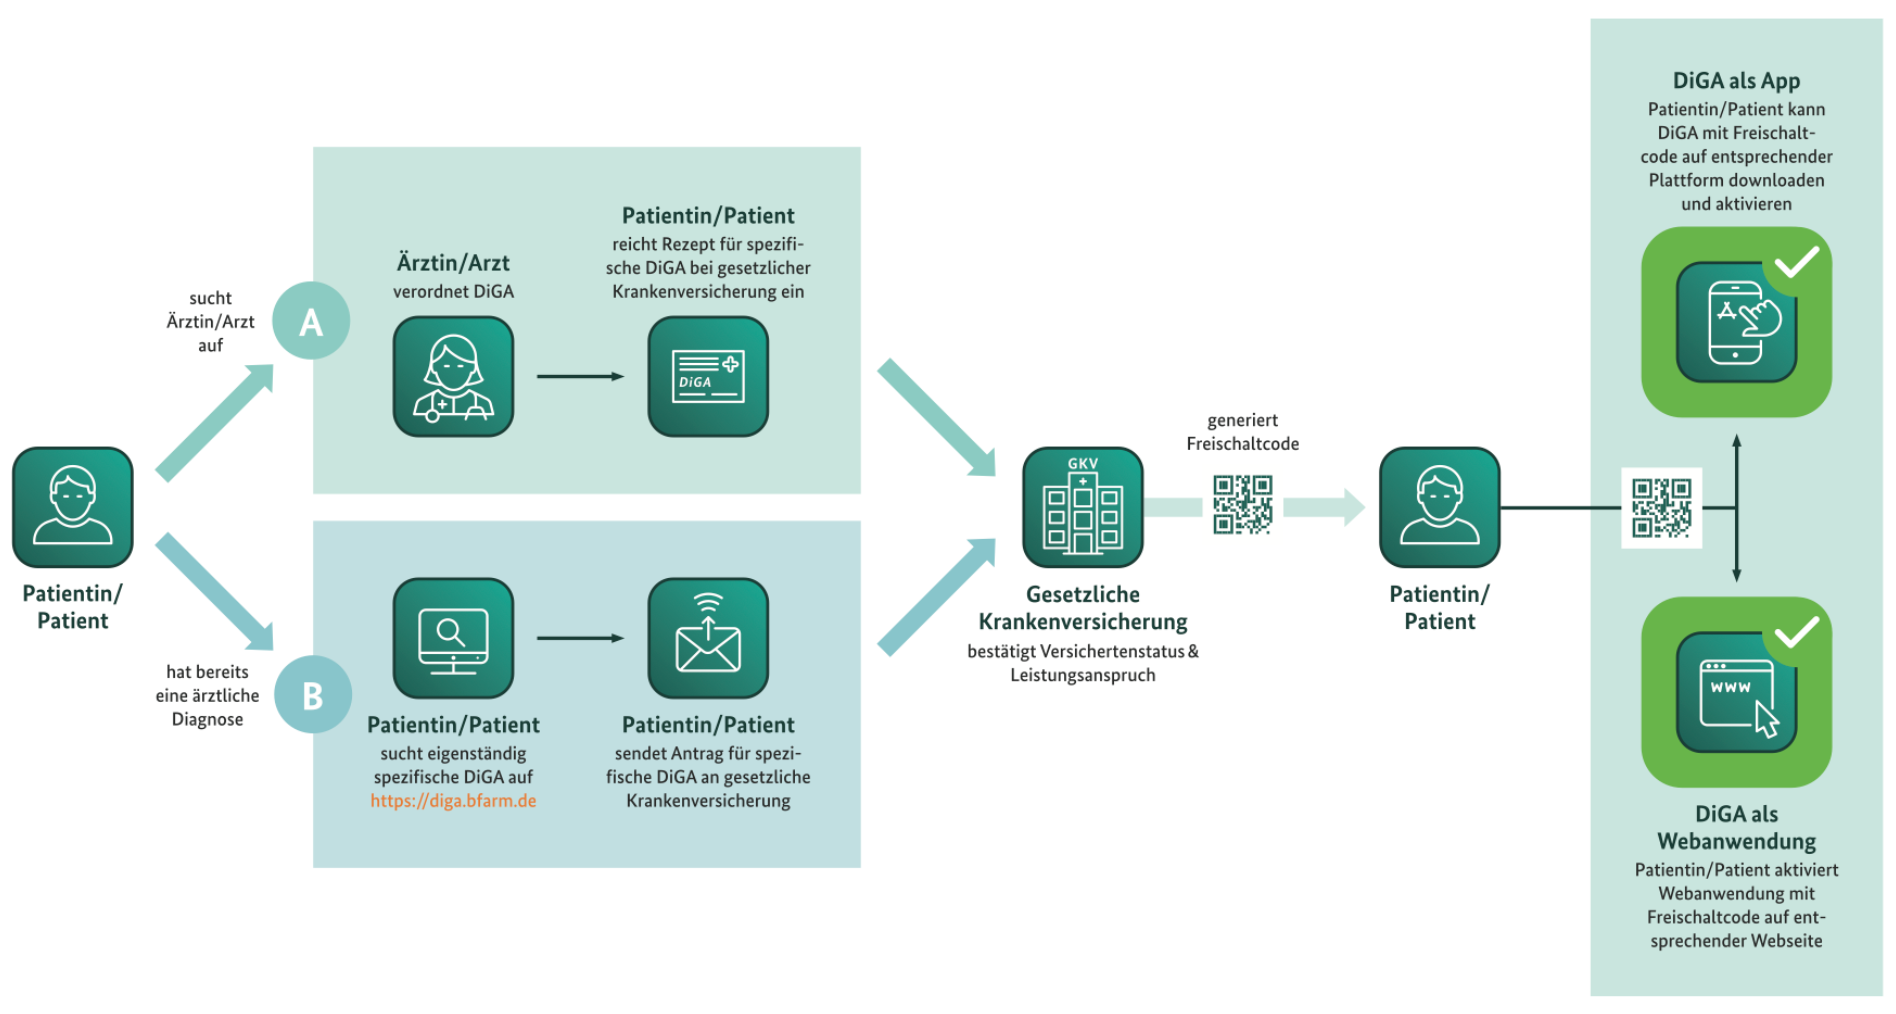
\includegraphics[width=450px, keepaspectratio]{assets/verordnungs_prozess.png}
	\caption{Graphauswertung - Komponentendiagramm,\\Quelle: Eigene Darstellung, Tool: \cite{visual_paradigm}}
\end{figure}
%Kern des Verfahrens sind die Prüfung der Herstellerangaben zu den geforderten Produkteigenschaften – vom Datenschutz bis zur Benutzerfreundlichkeit – sowie die Prüfung eines durch den Hersteller beizubringenden Nachweises für die mit der DiGA realisierbaren positiven Versorgungseffekte. Das sind Effekte, durch die sich der gesundheitliche Zustand eines Patienten oder die Möglichkeiten zum Umgang mit seiner Erkrankung durch die Benutzung der DiGA verbessern.
%
\begin{small}
\begin{quote}
"`Lorem ipsum dolor sit amet, consectetur adipisici elit, sed eiusmod tempor incidunt ut labore et dolore magna aliqua. Ut enim ad minim veniam, quis nostrud exercitation ullamco laboris nisi ut aliquid ex ea commodi consequat. Quis aute iure reprehenderit in voluptate velit esse cillum dolore eu fugiat nulla pariatur. Excepteur sint obcaecat cupiditat non proident, sunt in culpa qui officia deserunt mollit anim id est laborum."' (übersetzt durch Autor)\footnote{Bei Überzetzungen sollte genannt werden, ob es sich um eine in der Literatur rezipierte Übersetzung handelt, oder ob es sich um ein Eigenübersetzung des Autors handelt}
\end{quote}
\end{small}
%
Lorem ipsum dolor sit amet, consectetur adipisici elit, sed eiusmod tempor incidunt ut labore et dolore magna aliqua. Ut enim ad minim veniam, quis nostrud exercitation ullamco laboris nisi ut aliquid ex ea commodi consequat. Quis aute iure reprehenderit in voluptate velit esse cillum dolore eu fugiat nulla pariatur. Excepteur sint obcaecat cupiditat non proident, sunt in culpa qui officia deserunt mollit anim id est laborum.\\

\subsection{Wie funktioniert das Fast-Track- Verfahren?}

\begin{figure}[H]
	\centering
	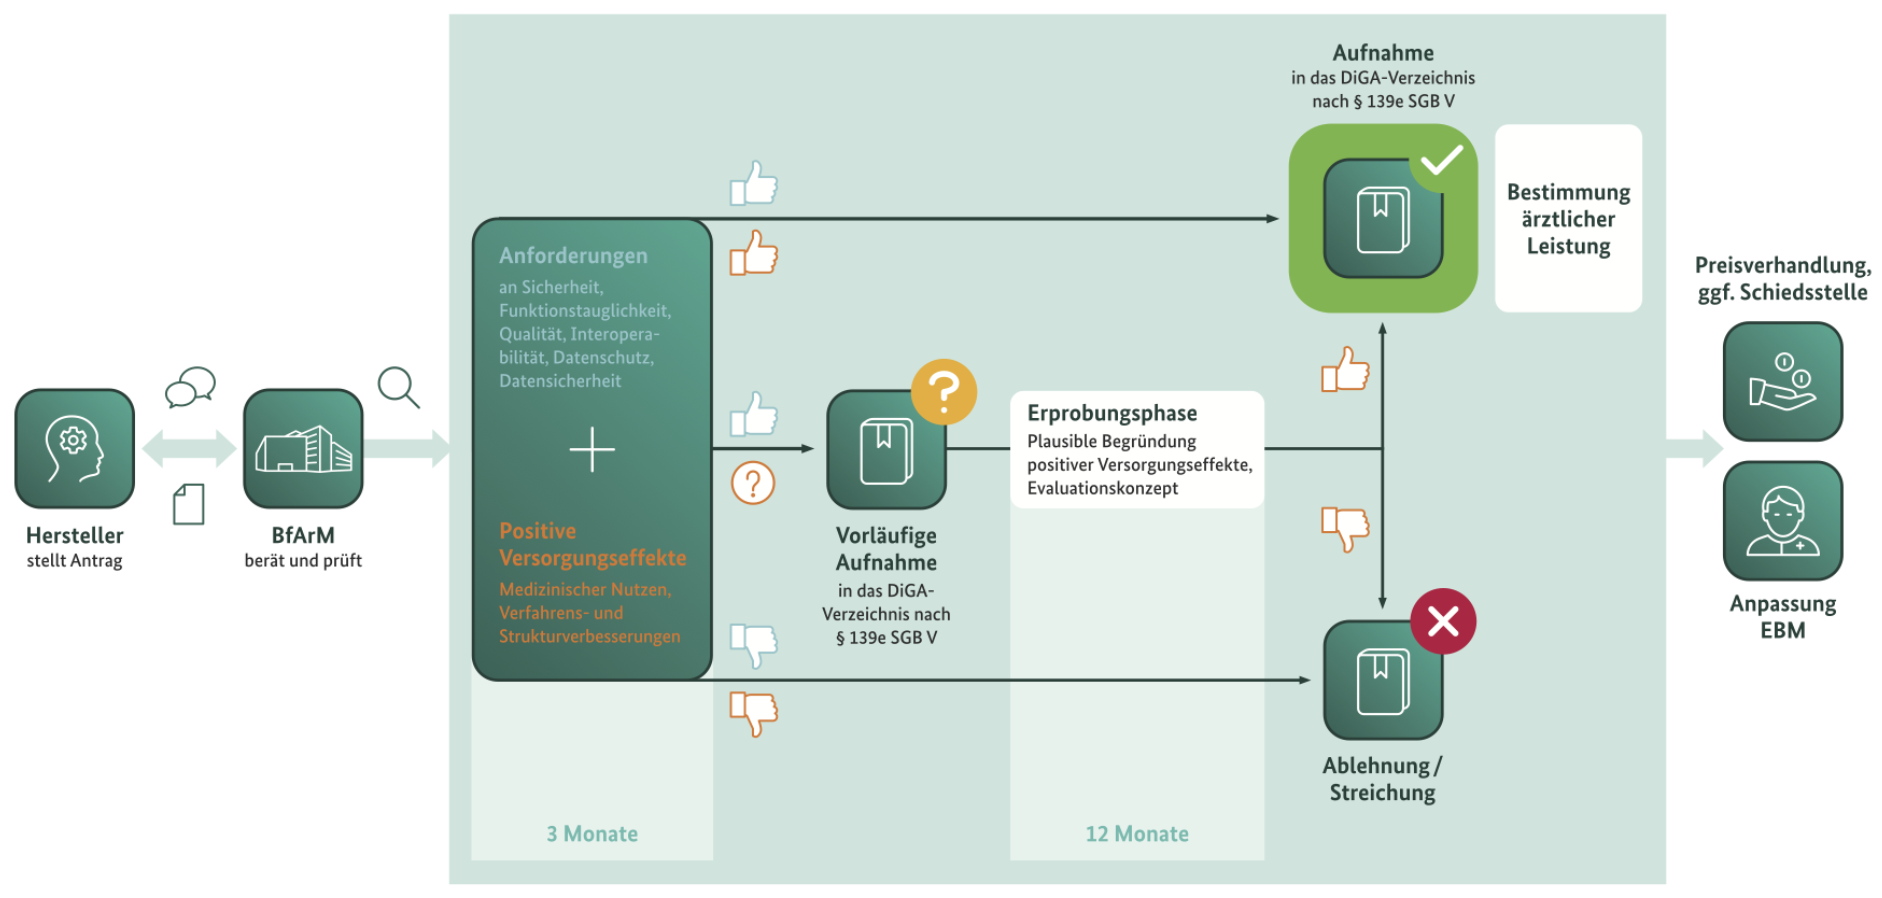
\includegraphics[width=450px, keepaspectratio]{assets/fastTrack_prozess.png}
	\caption{Graphauswertung - Komponentendiagramm,\\Quelle: Eigene Darstellung, Tool: \cite{visual_paradigm}}
\end{figure}
Lorem ipsum dolor sit amet, consectetur adipisici elit, sed eiusmod tempor incidunt ut labore et dolore magna aliqua. Ut enim ad minim veniam, quis nostrud exercitation ullamco laboris nisi ut aliquid ex ea commodi consequat. Quis aute iure reprehenderit in voluptate velit esse cillum dolore eu fugiat nulla pariatur. Excepteur sint obcaecat cupiditat non proident, sunt in culpa qui officia deserunt mollit anim id est laborum.

\subsection{Probleme bei der Analyse des Arbitrageverhaltens}
Lorem ipsum dolor sit amet, consectetur adipisici elit, sed eiusmod tempor incidunt ut labore et dolore magna aliqua. Ut enim ad minim veniam, quis nostrud exercitation ullamco laboris nisi ut aliquid ex ea commodi consequat. Quis aute iure reprehenderit in voluptate velit esse cillum dolore eu fugiat nulla pariatur. Excepteur sint obcaecat cupiditat non proident, sunt in culpa qui officia deserunt mollit anim id est laborum.\\
%
\begin{enumerate}
 \item Lorem ipsum
\item dolor sit amet, consectetur adipisici elit
\item sed eiusmod tempor incidunt ut labore et dolore magna aliqua
\end{enumerate}
%
Lorem ipsum dolor sit amet, consectetur adipisici elit, sed eiusmod tempor incidunt ut labore et dolore magna aliqua. Ut enim ad minim veniam, quis nostrud exercitation ullamco laboris nisi ut aliquid ex ea commodi consequat. Quis aute iure reprehenderit in voluptate velit esse cillum dolore eu fugiat nulla pariatur. Excepteur sint obcaecat cupiditat non proident, sunt in culpa qui officia deserunt mollit anim id est laborum.\footnote{Lorem ipsum dolor sit amet, consectetur adipisici elit, sed eiusmod tempor incidunt ut labore et dolore magna aliqua.} Lorem ipsum dolor sit amet, consectetur adipisici elit, sed eiusmod tempor incidunt ut labore et dolore magna aliqua. Ut enim ad minim veniam, quis nostrud exercitation ullamco laboris nisi ut aliquid ex ea commodi consequat. Quis aute iure reprehenderit in voluptate velit esse cillum dolore eu fugiat nulla pariatur. Excepteur sint obcaecat cupiditat non proident, sunt in culpa qui officia deserunt mollit anim id est laborum.